\section{Design overview}
\label{sec:matrix}

The objective of Matrix is to enable any-to-any routing in an
underlying data collection protocol for 6LoWPAN, such as CTP and
RPL, while preserving memory and message efficiency, as well as
adaptability to networks topology dynamics\footnote{Note that Matrix
is not designed to address scenarios with node mobility, but only to
work with network topology dynamics caused by changes in link
quality, as well as node and link failures.}. Matrix is a network
layer protocol that works together with a routing protocol.
Figure~\ref{fig:architecture} illustrates the protocol's
architecture, which is divided into: \textit{routing engine} and
\textit{forwarding engine}. The routing engine is responsible for
the address space partitioning and distribution, as well as routing
table maintenance. The forwarding engine is responsible for
application packet forwarding.

\begin{figure}[!ht]
    \centering
    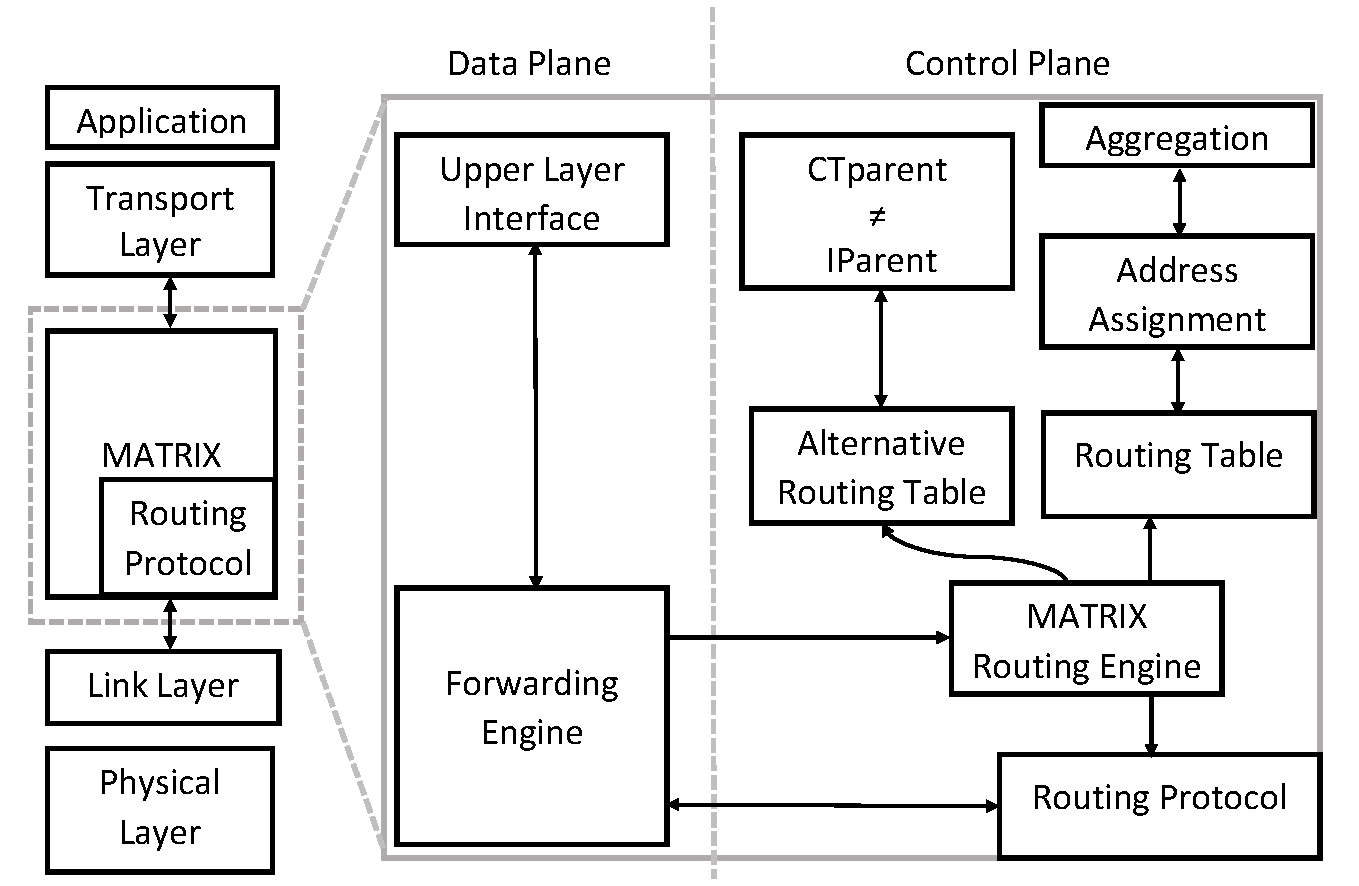
\includegraphics[width=1\columnwidth]{./Images/Architecture.pdf}
\caption{Matrix protocol's architecture.}
    \label{fig:architecture}
\end{figure}

Matrix is comprised of the following execution phases:
\begin{enumerate}
  \item \textbf{Collection tree initialization}: the
  collection tree (Ctree) is built by the underlying collection protocol; each
  node achieves a stable knowledge about who its parent is; adaptive beaconing
  based on Trickle algorithm \cite{Levis:2004} is used to define stability;
  
 \item \textbf{IPv6 multihop host configuration}: once the collection tree
  is stable, the address hierarchy tree (IPtree) is built using MHCL
  (Section~\ref{subsec:mhcl}); this phase also uses adaptive beaconing to handle network
  dynamics; by the end of this phase, each node has received an IPv6 address
  range from its parent and each non-leaf node has partitioned its own address 
	space among its children; the resulting address
  hierarchy is stored in the distributed IPtree, which initially has the same
  topology as Ctree, but in reverse, top-down, direction.
  
\item \textbf{Standard routing}: bottom-up routing is done
  using the collection tree, Ctree, and top-down routing is done using the
  address hierarchy represented by the IPtree; any-to-any routing is performed by combining
  bottom-up forwarding, until the least common ancestor of sender and
  receiver, and then top-down forwarding until the destination.
  
\item \textbf{Alternative top-down routing table upkeep}: whenever a node changes its parent in the initial collection tree, it starts sending beacons to its new parent in Ctree, requesting to upkeep an entry in its routing table with its own IPv6 range; such new links in Ctree, in reverse direction, comprise the RCtree routing tables for alternative (top-down) routing;

\item \textbf{Alternative top-down routing via local broadcast}:
whenever a node fails to forward a data packet to the next hop/subtree in the IPtree, it
  broadcasts the packet to its one-hop neighborhood; upon receiving a local
  broadcast, all neighbors check if the destination IPv6 belongs to an address
  range in their RCtree table; if positive, the packet is forwarded to the
  correct subtree of IPtree, otherwise, the packet is dropped; we give a
  geometric argument and show through simulations that such events are rare.
\end{enumerate}

Next we describe the architecture of Matrix in more detail.

\subsection{MHCL: Multihop Host Configuration for 6LoWPAN}
\label{subsec:mhcl}

Matrix is built upon the idea of IPv6 hierarchical address allocation. The address space available to the border router of the 6LoWPAN (e.g., the 64 least-significant bits of the IPv6 address or a compressed 16-bit representation of it) is hierarchically partitioned among nodes connected to the border router through a multihop cycle-free topology (implemented by standard protocols, such as RPL or CTP). Each node receives an address range from its parent and partitions it among its children, until all nodes receive an address. Since the address allocation is performed in a hierarchical way, the routing table of each node has $k$ entries, where $k$ is the number of its (direct) children. Each routing table entry aggregates the addresses of all nodes in the subtree rooted at the corresponding child-node. A portion, say $r\%$, of the address space available to each node is left reserved for possible future/delayed connections (parameter $r$ can be configured according to the expected number of newly deployed nodes in the network, see Figure~\ref{fig:addrPartitionAggregate}). We refer to the resulting distributed tree structure as IPtree.


\textbf{Messages:} MHCL uses two message types: $MHCL_{A}$ ($MHCL_{Aggregation}$) e $MHCL_{D}$ ($MHCL_{Distribution}$). 
Messages of type $MHCL_{A}$ are used in the upward routes, from child to parent. This message carries the number of a node's descendants, used in the aggregation phase. Messages of type $MHCL_{D}$ are sent along downward routes, from parent to child. This message is used for address allocation and contains the address and corresponding address partition assigned to a child node by its parent. Note that the size of the first address and the size of the allocated address partition can have a length predefined by the root, according to the overall address space (we used a value of 16 bits, because the compressed host address has 16 bits). This information is sufficient for the child node to decode the message and execute the address allocation procedure for its children.


\textbf{Network stabilization:} In order to decide how the available address space is partitioned, nodes need to collect information about the topology of the network. Once a \textit{stable} view of the network's topology is achieved, the root starts distributing address ranges downwards to all nodes. Note that the notion of stability is important to implement a coherent address space partition. Therefore, MHCL has an initial set-up phase, during which information about the topology is progressively updated, until a (predefined) sufficiently long period of time goes by without any topology changes. To implement this adaptive approach, we use Trickle-inspired timers to trigger messages (Algorithm \ref{alg:stabilization}). In Algorithm \ref{alg:stabilization} two parameters are used: $Trickle_{min}$ is the minimum time interval used by the Trickle algorithm, and $spChild$ is a multiplication factor used to define the maximum time interval, such that, if no changes occur within it, then the parent choice becomes
  stable, and the local variable $parentDefined$ is set to TRUE.  Note that, once the network reaches an initial state of stability, later changes to topology are expected to be of local nature, caused by a link or a node failure, or a change in the preferred parent of a node. In these cases, the address allocation does not need to be updated, since local mechanisms of message resubmission can be used to improve message delivery rates, as described in Section~\ref{subsec:localBroadcast}.

\begin{algorithm}[h]
\caption{MHCL: Stabilization timer}\label{alg:stabilization}
\begin{algorithmic}[1]
\State parentDefined = FALSE;
\State maxTime = $spChild * Trickle_{min}$ ;
\State timer = rand($1/2 * Trickle_{min}$, $Trickle_{min}$]; \Comment{reset timer}
\While{NOT parentDefined}
	\If {NOT-ROOT \textbf{and} TIMER-OFF}
		\If {PARENT-CHANGED}
			\State reset timer;
		\Else	
		\If {$timer < maxTime$}
			\State timer *= 2; \Comment{double timer}
		\Else
			\State parentDefined = TRUE;
		\EndIf
		\EndIf
	\EndIf	
\EndWhile
\end{algorithmic}
\end{algorithm}

\begin{figure}
\centering
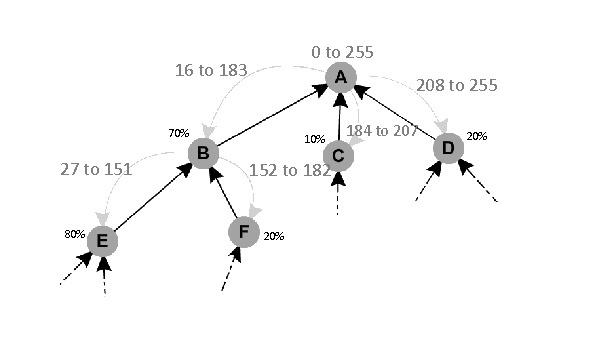
\includegraphics[width=.7\columnwidth]{Images/mhcl-a.pdf}
\caption{MHCL: simplified IPtree example: 8-bit address space at the root and $6.25\%$ reserved for future/delayed connections.}\label{fig:addrPartitionAggregate}
\end{figure}

\textbf{Descendants convergecast:} After the initial network stabilization, each node $n_i$ counts the total number of its descendants, i.e., the size of the subtree rooted at itself, and propagates it to its parent. Moreover, $n_i$ saves the number of descendants of each child. If a node is not the root, and it has defined who the preferred parent is ($parentDefined$ is TRUE) it starts by sending a $MHCL_{A}$ message with $count=0$ (Algorithm~\ref{alg:bottomUpNotRoot}). Then it waits for $MHCL_{A}$ messages from its children, updates the number of descendants of each child, and propagates the updated counter to the parent until its total number of descendants is stable. If a node is the root, then it just updates the number of descendants of each child by receiving  $MHCL_{A}$ messages until its total number of descendants is stable (Algorithm \ref{alg:bottomUpRoot}). Parameters $spLeaf$ and $spRoot$ are used to define stabilization criteria in non-root nodes and the root node, respectively. Once the aggregation phase is completed, the root's local variable $descendantsDefined$ is set to TRUE.

\begin{algorithm}[h!]
\caption{MHCL: Aggregation
timer (non-root nodes)}\label{alg:bottomUpNotRoot} 
\begin{algorithmic}[1]
  \State maxTimeLeaf = $spLeaf*Trickle_{min}$; 
  \State timer = rand($1/2 * Trickle_{min}$, $Trickle_{min}$]; \Comment{reset timer}
  \State count = 0; \Comment{counts descendants through $MHCL_{A}$ messages}
\While{NO-$MHCL_{D}$-FROM-PARENT} 
\State \Comment{hasn't received IPv6 range}
\If{NOT-ROOT \textbf{and} TIMER-OFF}
		\If{parentDefined \textbf{and} $(count<1)$}
			\State send $MHCL_{A}$ to parent; \Comment{trigger aggregation}
		\EndIf
		\If {COUNT-CHANGED}
			\State send $MHCL_{A}$ to parent; 
			\State reset timer;		
		\Else	\If{$timer < maxTimeLeaf$} %param=4
					\State timer *= 2;
				\EndIf
		\EndIf
\EndIf
\EndWhile
\end{algorithmic}
\end{algorithm}

\begin{algorithm}[h!]
\caption{MHCL: Aggregation timer (Root)}\label{alg:bottomUpRoot}
\begin{algorithmic}[1]
  \State descendantsDefined = FALSE;	
  \State maxTimeRoot = $spRoot *Trickle_{min}$; 
  \State timer = rand($1/2 * Trickle_{min}$, $Trickle_{min}$]; \Comment{reset timer}
  \State count = 0; \Comment{counts descendants through $MHCL_{A}$ messages}
\While{NOT descendantsDefined}
\If{IS-ROOT \textbf{and} TIMER-OFF}
		\If{COUNT-CHANGED} %\textbf{or} $(count<1)$
			\State reset timer;
		\Else
			\If{$timer < maxTimeRoot$}
				\State $timer *= 2$;
			\Else
				\State descendantsDefined = TRUE;
			\EndIf
		\EndIf
\EndIf
\EndWhile
\end{algorithmic}
\end{algorithm}

\textbf{Address allocation:} Once the root has received the (aggregate) number of descendants of each child, it partitions the available address space into $k$ ranges of size proportional to the size of the subtree rooted at each child (see Algorithm~\ref{alg:addrDistr}). Each node $n_i$ repeats the space partitioning procedure upon receiving its own address space from the parent and sends the proportional address ranges to the respective children (always reserving $r\%$ for delayed address allocation requests). The idea is to allocate larger portions to larger subtrees, which becomes important in especially large networks, because it maximizes the address space utilization. Note that this approach needs information aggregated along multiple hops, which results in a longer set-up phase.

\textbf{Delayed connections:} If an address allocation request from a new child node is received after the address space had already been partitioned and assigned, then the address allocation procedure is repeated using the reserved address space.
  
\begin{algorithm}[h!]
\caption{MHCL: IPv6 address distribution}\label{alg:addrDistr}
\begin{algorithmic}[1]
 \State STABLE = descendantsDefined \textbf{or} NOT-ROOT;		
  \If {STABLE \textbf{and} (IS-ROOT \textbf{or} RECEIVED-$MHCL_{D}$)} 
  	\State partition available address space;
	\For{each child $c_i$} 
		\State send $MHCL_{D}$ to $c_i$; \Comment{send IPv6 ``range''}
		\If{NO $ack$}
			\State send $MHCL_{D}$ to $c_i$; \Comment{retransmit}
		\EndIf
  	\EndFor		
  \EndIf
\end{algorithmic}
\end{algorithm}

After the address allocation is complete, each (non-leaf) node stores a routing table for downward traffic, with an entry for each child. Each table entry contains the final address of the address range allocated to the corresponding child, and all table entries are sorted in increasing order of the final address of each range. In this way, message forwarding can be performed in (sub)linear time. 



\subsection{Control plane: distributed tree structures}

After the network is initialized and all nodes have received an IPv6
address range, three simultaneous distributed trees are maintained
on all nodes in the 6LoWPAN: \textbf{Ctree:} the collection tree, maintained by the underlying collection protocol (CTP/RPL).
	\textbf{IPtree:} the IPv6 address tree, built during the network
  initialization phase and kept static afterwards, except when new
  nodes join the network, in which case they receive an IPv6 range from the reserve space of the respective
parent node in the collection tree.

	\textbf{RCtree:} the reverse collection tree, reflecting the
  dynamics of the collection tree in the reverse direction.

Initially, IPtree has the same topology as the reverse-collection tree
$Ctree^{R}$, and RCtree has no links (see Figure \ref{fig:t1} and
\ref{fig:t2}).
$$
IPtree = Ctree^{R} \ \text{and} \ RCtree = \emptyset
$$
Whenever a change occurs in one of the links in Ctree, the new link
is added in the reverse direction into RCtree and maintained as long
as this topology change persists (see Figures \ref{fig:t3} and
\ref{fig:t4}).
$$
RCtree = Ctree^{R} \setminus IPtree
$$

Therefore, RCtree is not really a tree since it contains only the
reversed links present in Ctree but not in IPtree. Nevertheless, its
union with the ``working'' links in IPtree is, in fact, a tree,
which is used in the alternative top-down routing:
$$
RCtree \cup (IPtree \cap Ctree^{R}) \  \text{:alternative routing tree.}
$$

\begin{figure}[!h]
\begin{center}
  \subfigure[]
  {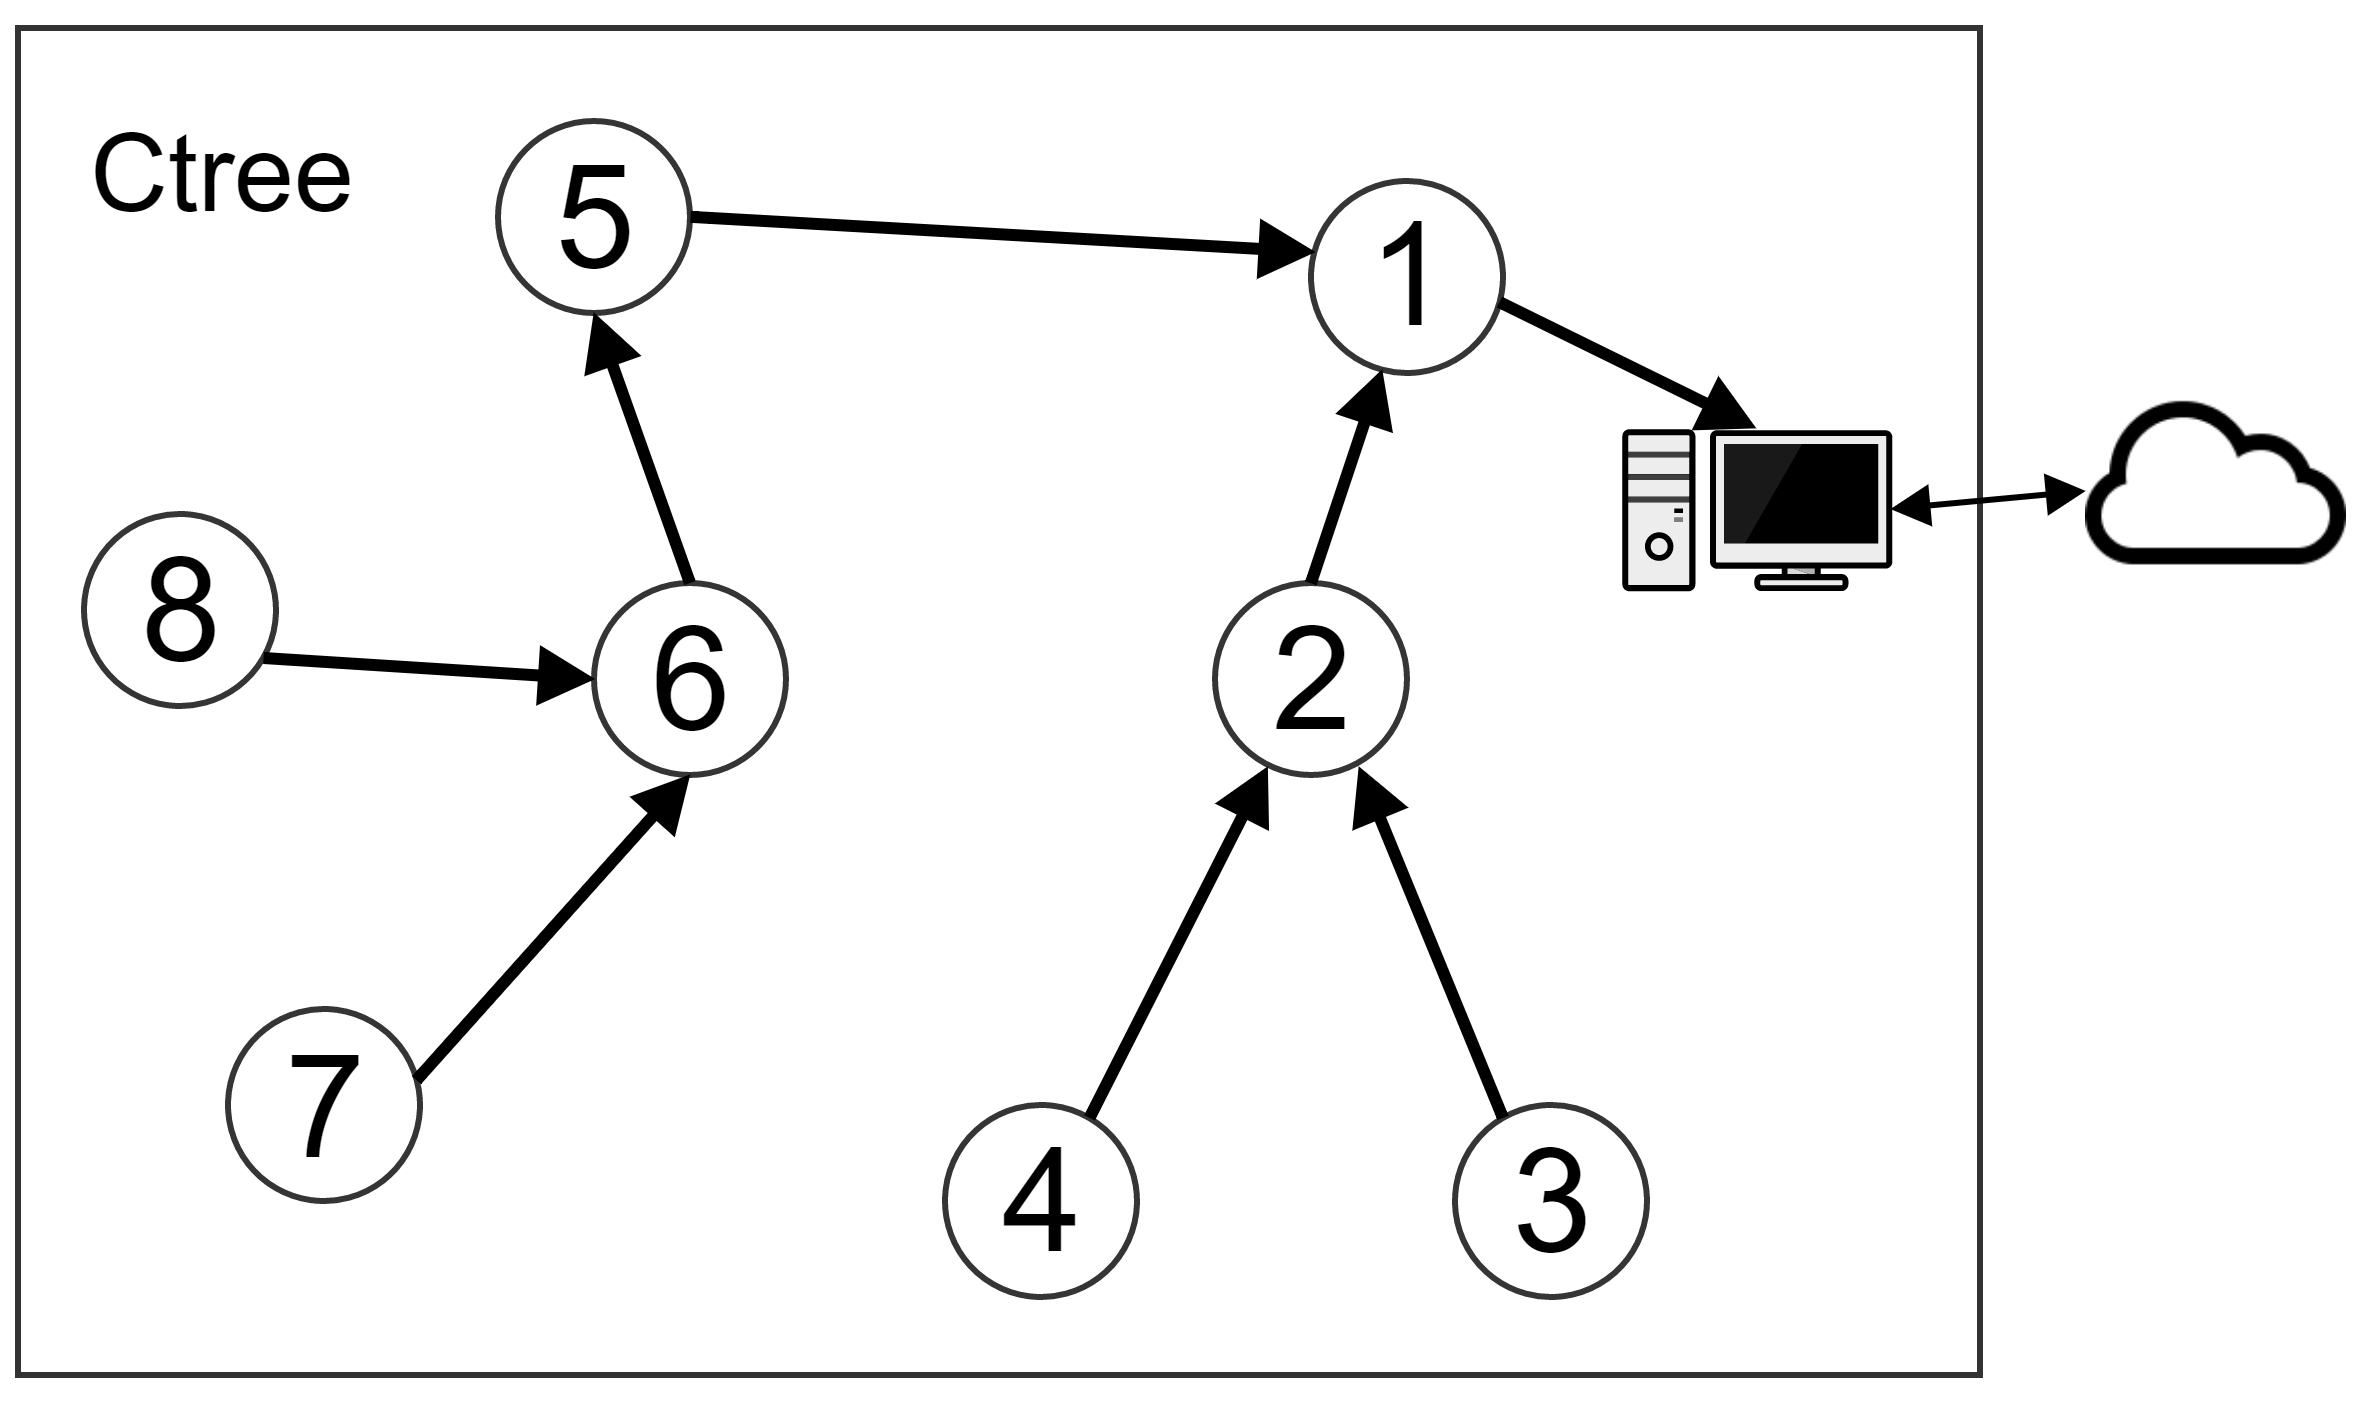
\includegraphics[width=.48\columnwidth]{Images/topologia1.jpg}
            \label{fig:t1}}
  \subfigure[]
  {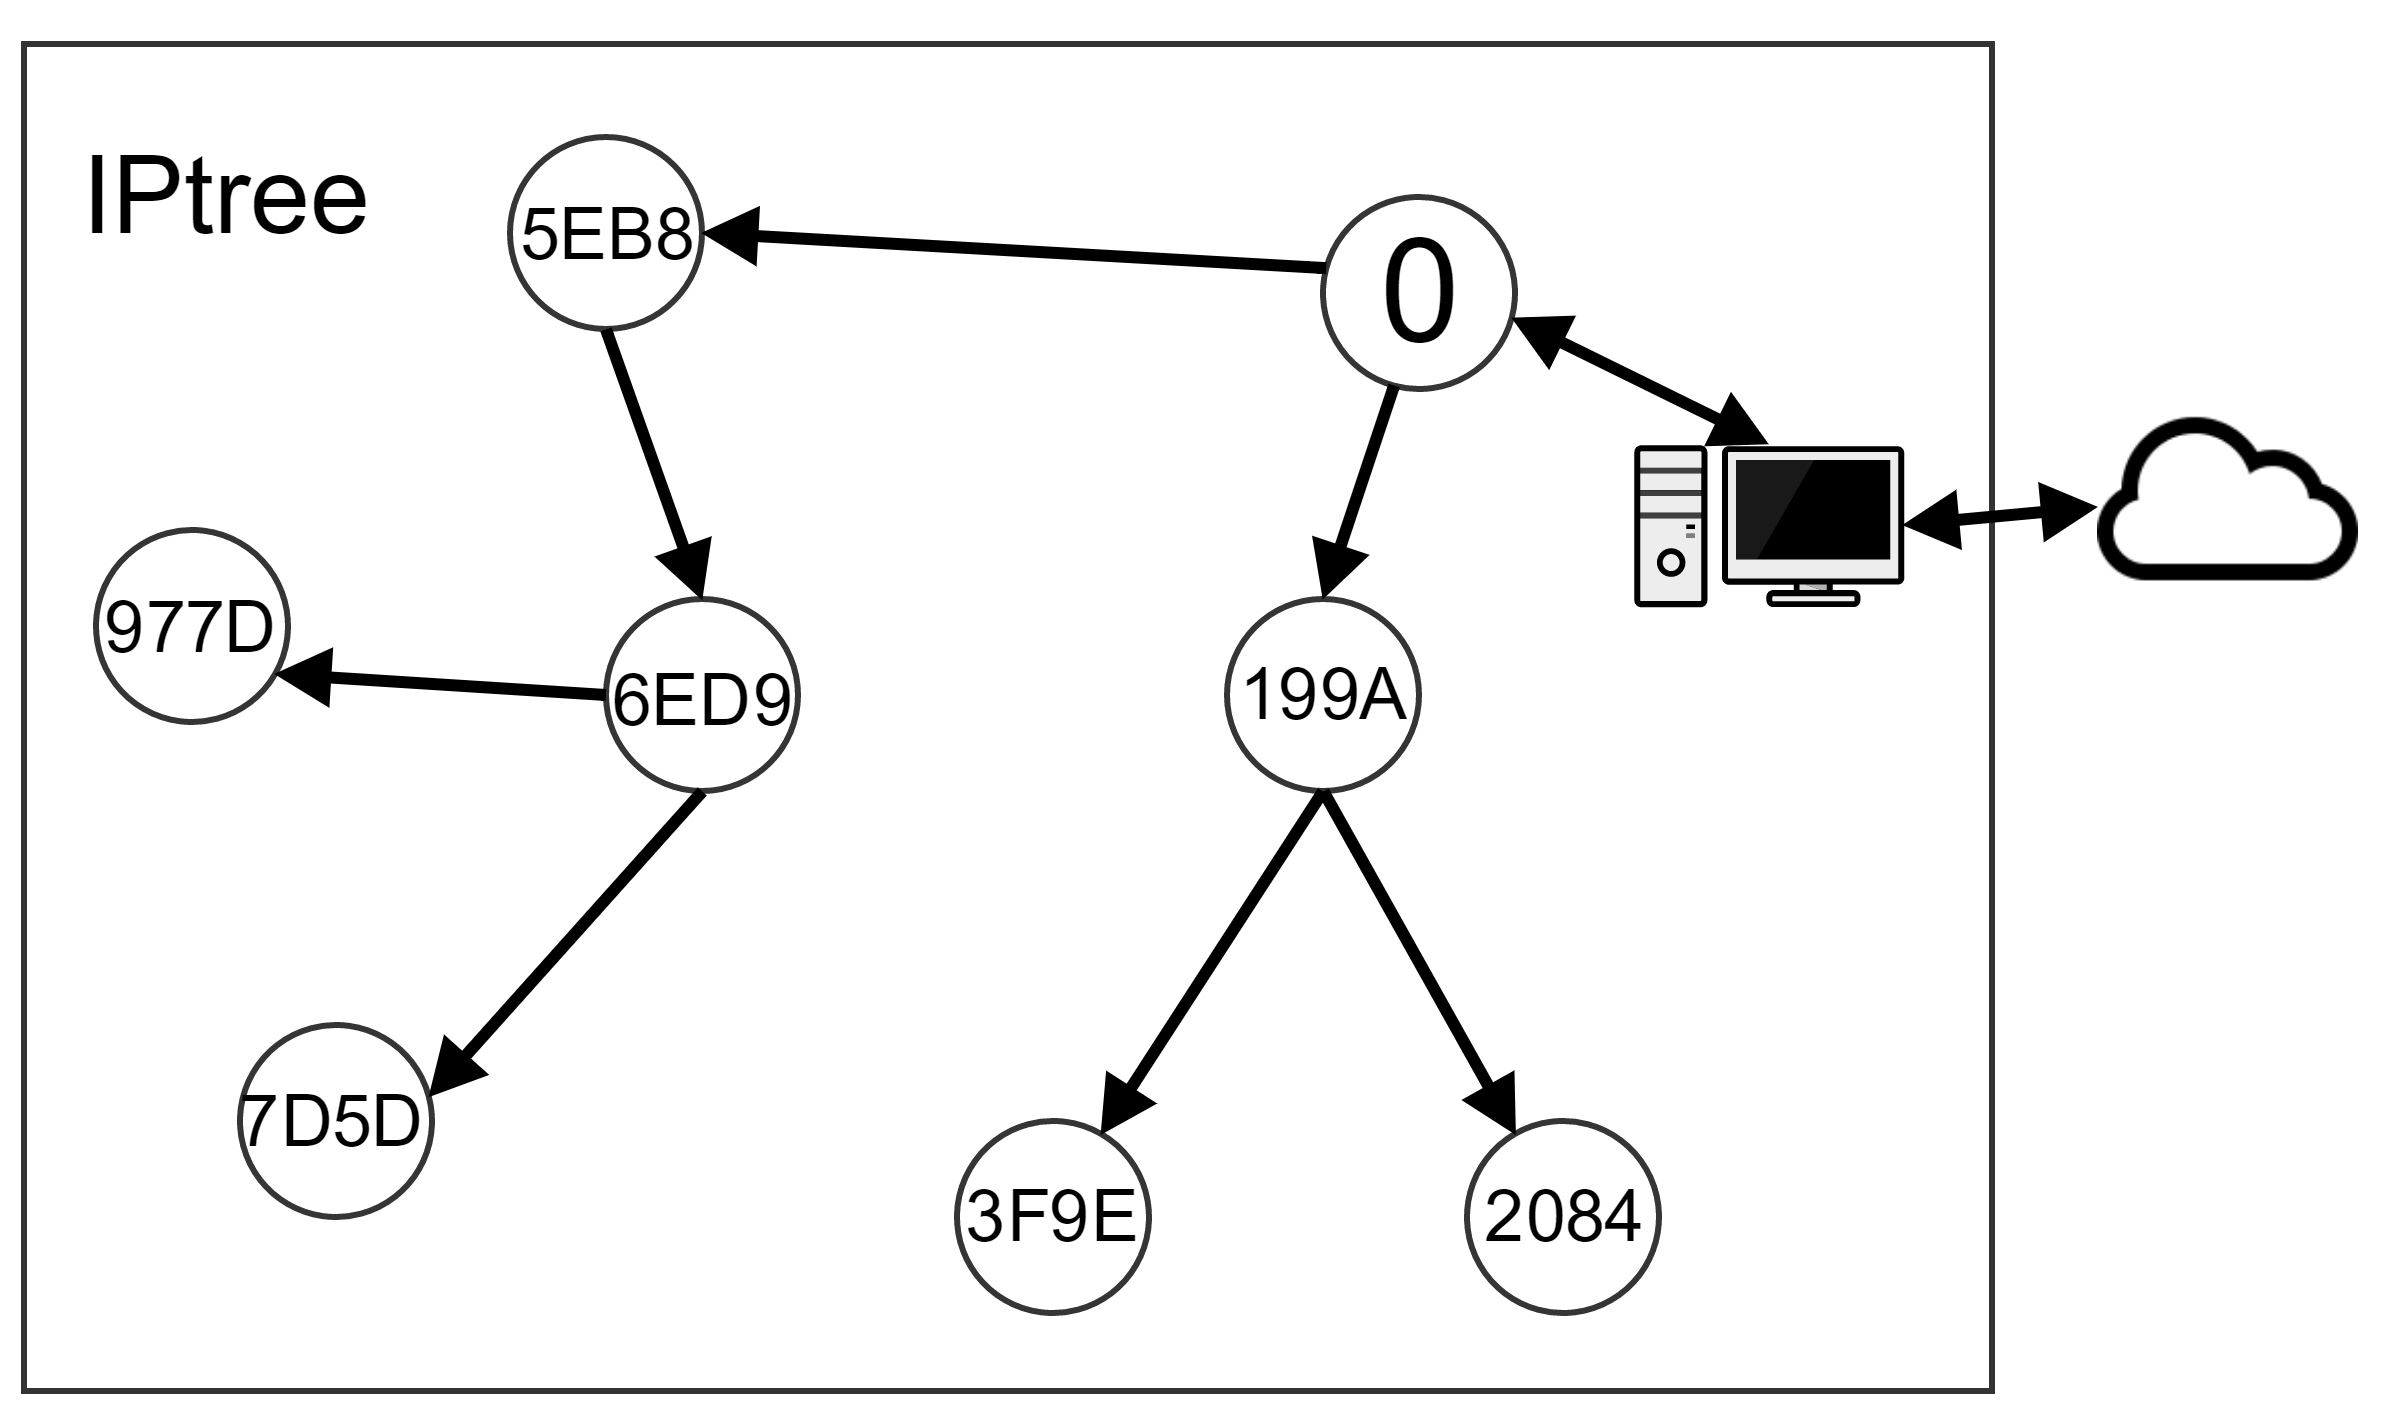
\includegraphics[width=.48\columnwidth]{Images/topologia2.jpg}
                        \label{fig:t2}}
                            \subfigure[]
  {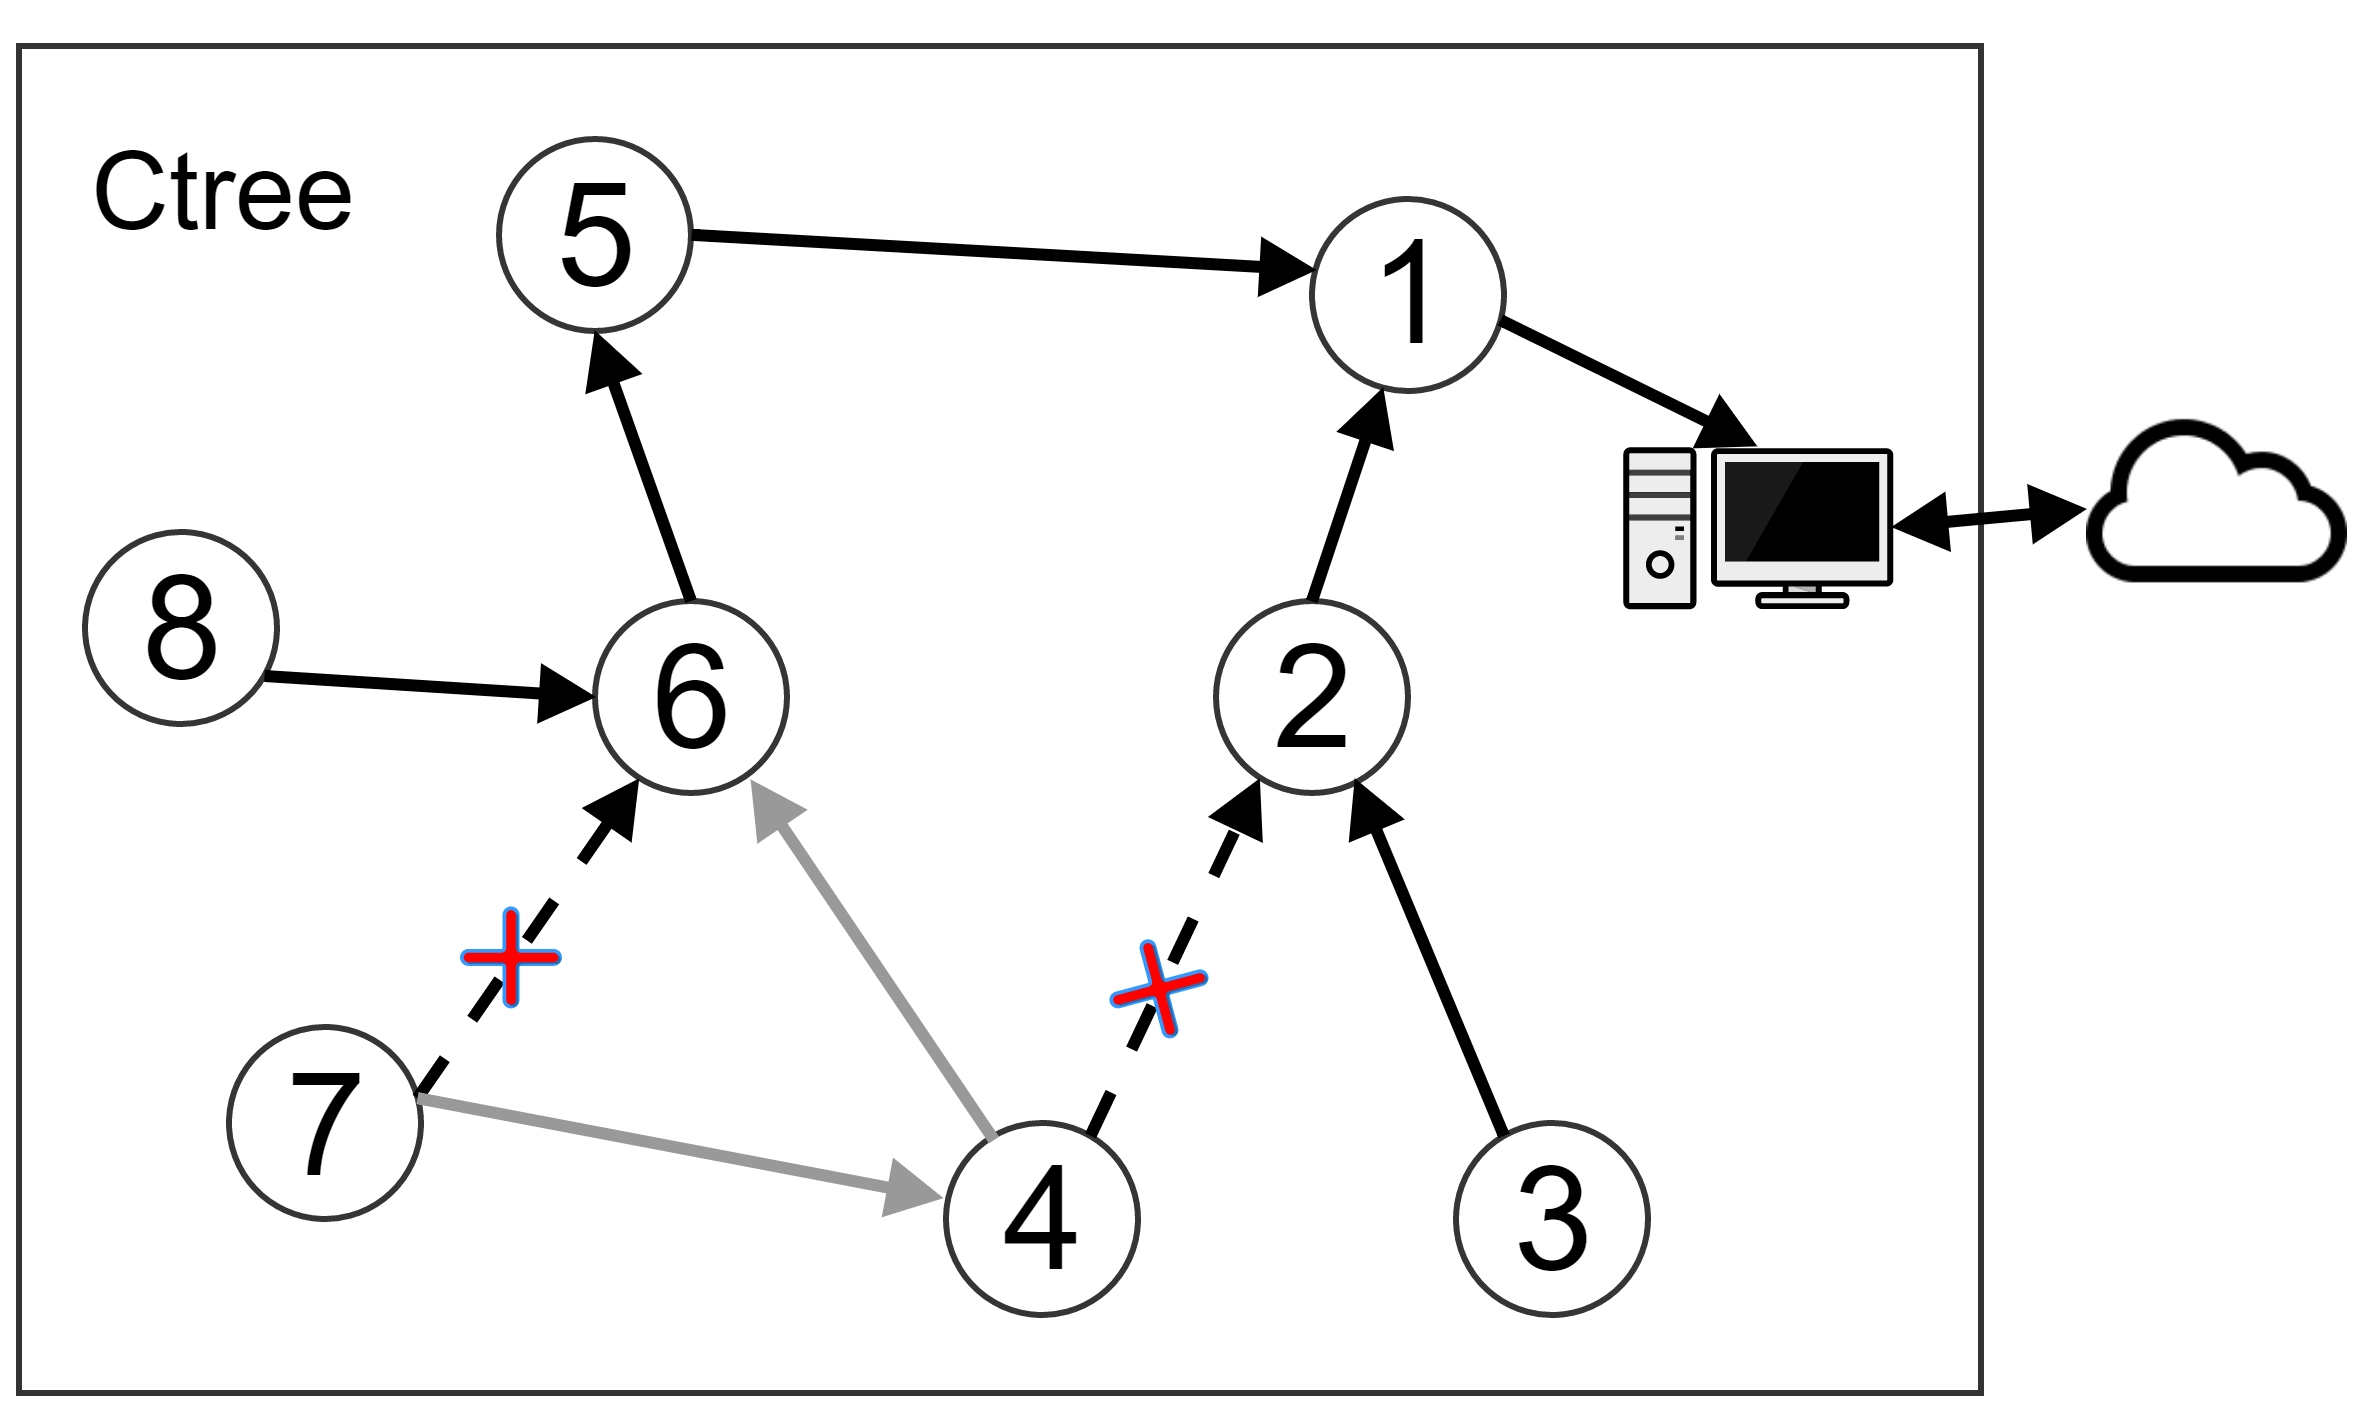
\includegraphics[width=.48\columnwidth]{Images/topologia3.jpg}
            \label{fig:t3}}
  \subfigure[]
  {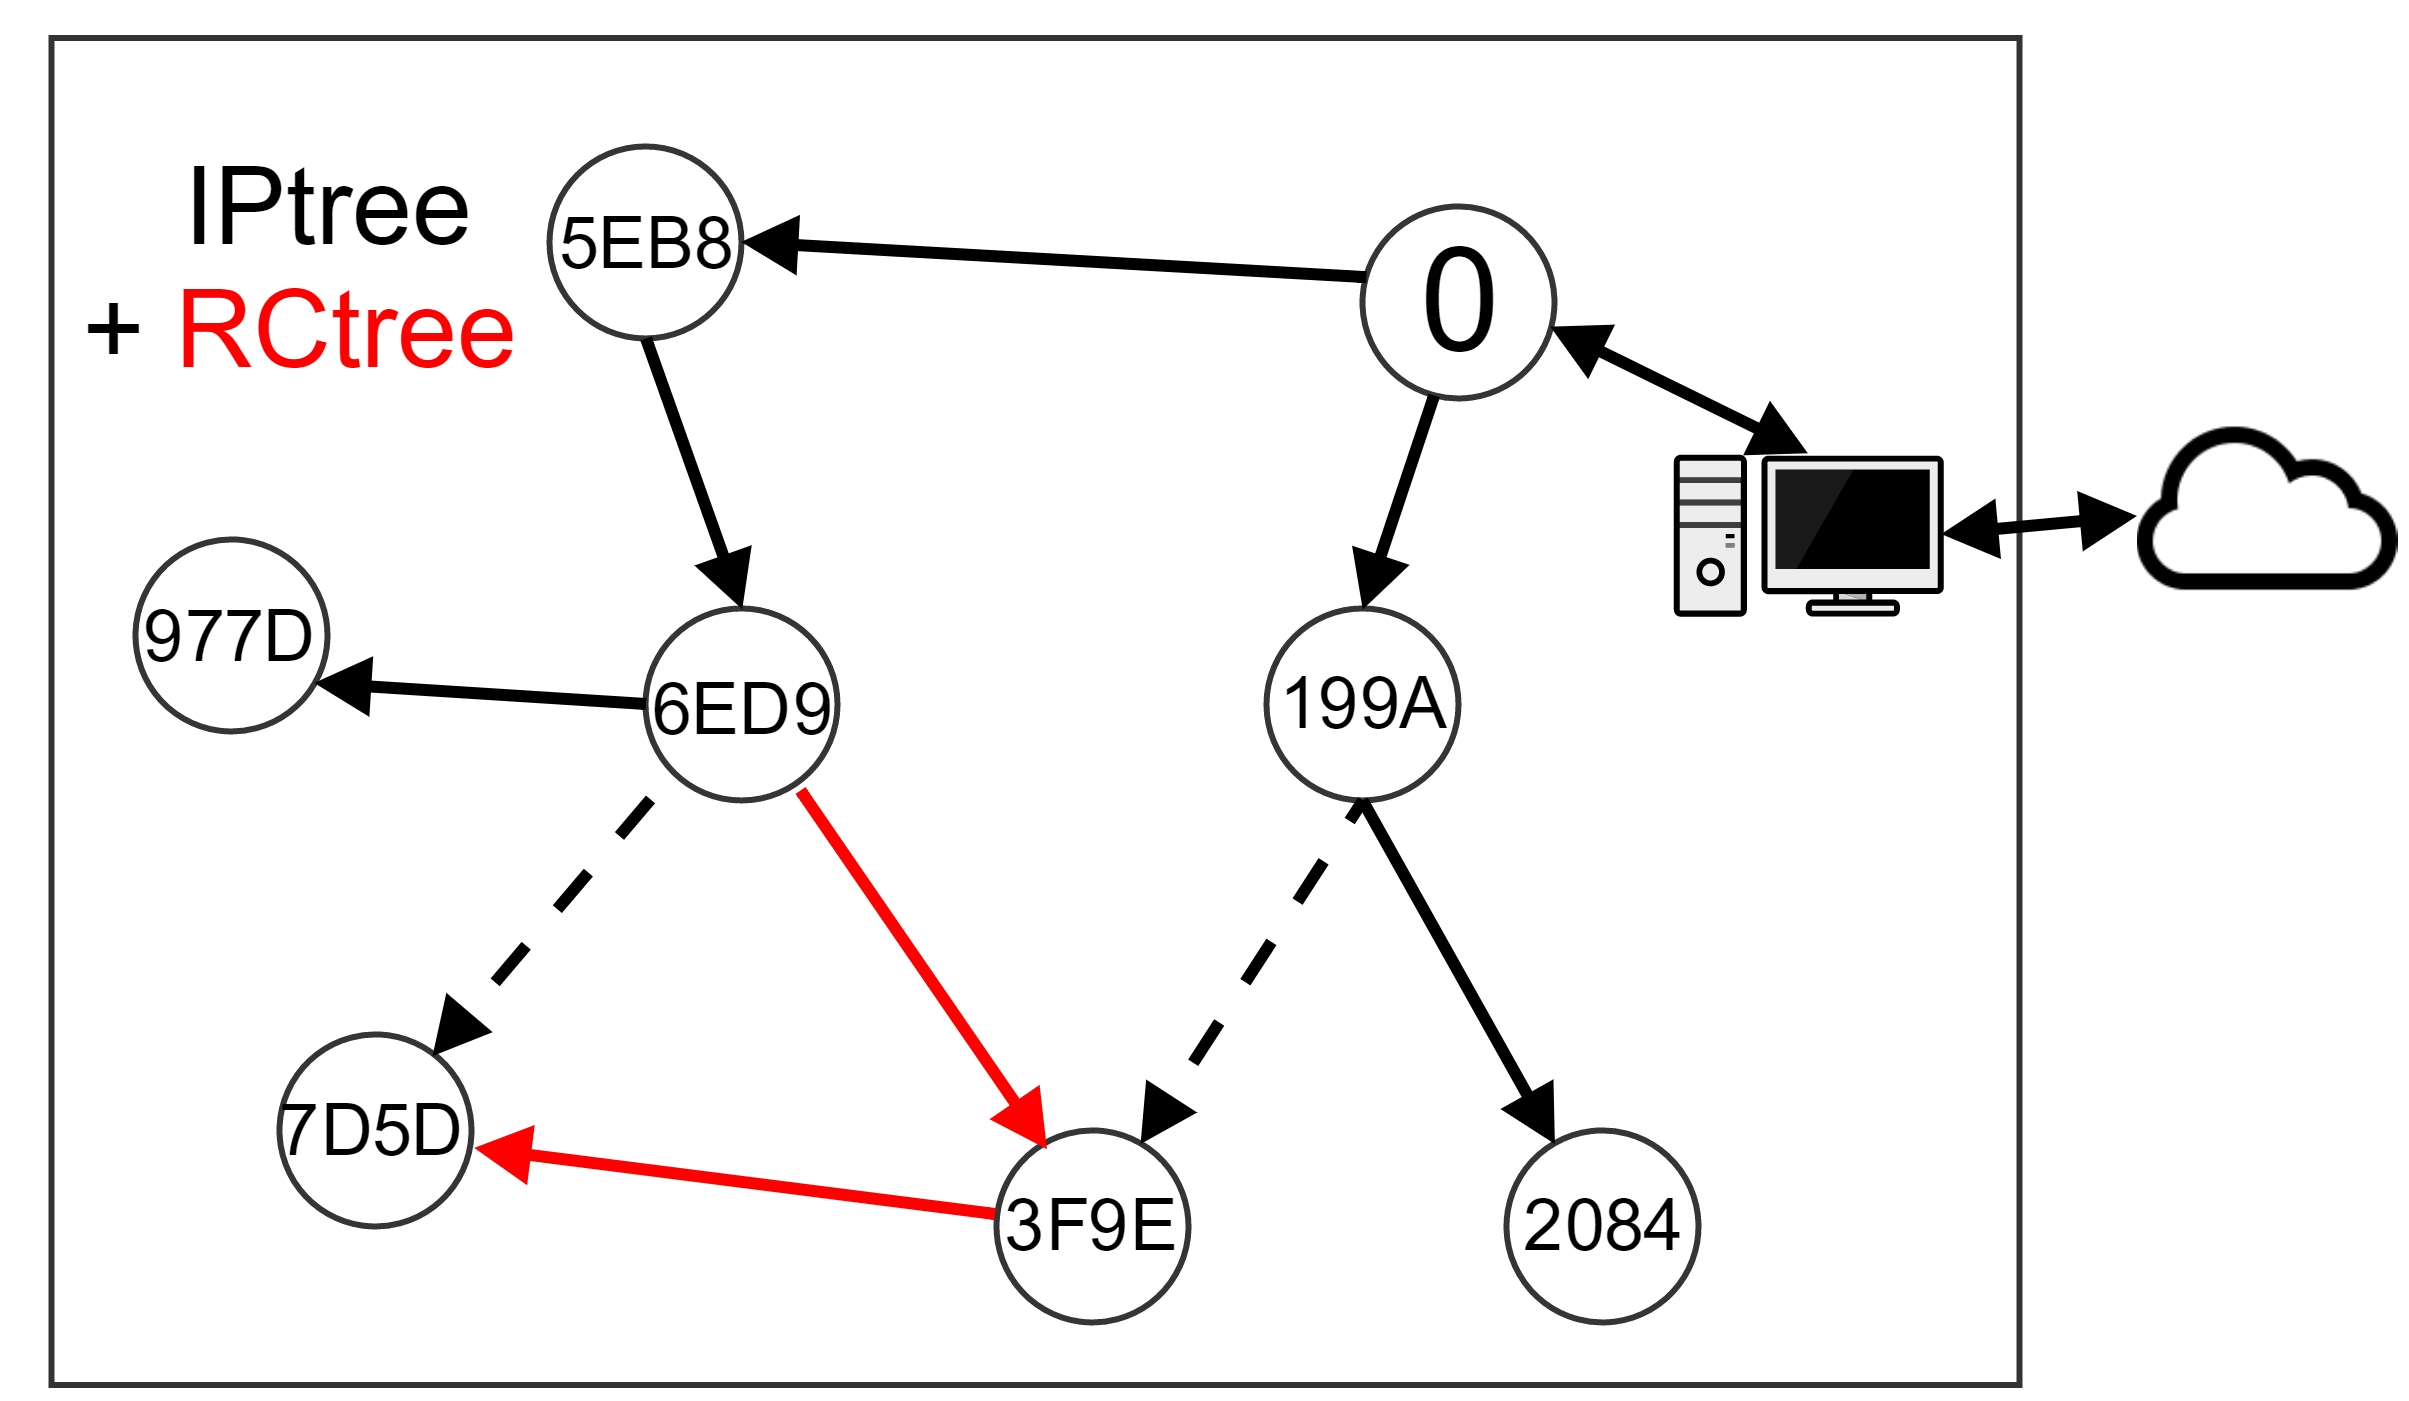
\includegraphics[width=.48\columnwidth]{Images/topologia4.jpg}
    \label{fig:t4}}
            \caption{RCtree example: before
            and after two links change in the collection tree.}\label{fig:layers}
\end{center}
\end{figure}

Each node $n_i$ maintains the following information:
\begin{itemize}
  \item $CTparent_i$: the ID of the current parent in the dynamic
  collection tree;
  \item $IParent_i$: the ID of the node that assigned $n_i$ its IPv6 range
initially $CTarent_i$ = $IParent_i$);
  \item $IPchildren_i$: the \textit{standard} (top-down) routing table, with
  address ranges of each one-hop descendant of $n_i$ in the IPtree;
  \item $RChildren_i$: the \textit{alternative} (top-down) routing table, with
  address ranges of one-hop descendants in the RCtree.
\end{itemize}

Note that, each node stores only one-hop
neighborhood information, so the memory footprint is $O(k)$, where $k$ is the
number of a node's children at any given moment in time, which is optimal,
considering that any (optimal) top-down routing mechanism would need at
least one routing entry for every (current) child in the tree topology to reach
all destinations.

The routing engine (see Figure~\ref{fig:architecture}) is responsible for
creating and maintaining the IPtree and RCtree routing tables. IPtree is created
during the network initialization phase, while RCtree is updated dynamically to
reflect changes in the network's link qualities. Whenever a node $n_i$ has its
$CTparent_i$ updated, and the current parent is different from its
$IParent_i$ ($IParent_i \neq CTparent_i$), $n_i$ starts sending periodic beacons
to its new parent, with regular intervals (in our experiments, we set the beacon
interval to $\delta/8$, where $\delta$ is the maximum interval of the
Trickle timer used in CTP).
Upon receiving a beacon (from a new child in the collection tree), a node
($n_j = CTparent_i$) creates and keeps an entry in its alternative
routing table $RChildren_j$ with the IPv6 address range of the subtree of $n_i$. As soon as $n_i$
stops using $n_j$ as the preferred parent, it stops sending beacons to $n_j$.
If no beacon is received from $n_i$ after $2\times\delta$ ms, its (alternative)
routing entry is deleted. Therefore, links in RCtree are temporary and are deleted when not present in neither the collection nor the IP trees.

\subsection{Data plane: any-to-any routing}

The forwarding engine (see Figure~\ref{fig:architecture}) is responsible for
application packet forwarding. Any-to-any routing is performed by combining
  bottom-up forwarding, until the least common ancestor of sender and
  receiver, and then top-down forwarding until the destination. Upon receiving
  an application layer packet, each node $n_i$ verifies whether the destination IPv6 address falls within some range
$j \in IPchildren_i$: if yes then the packet is forwarded
(downwards) to node $n_j$, otherwise, the packet is forwarded
(upwards) to $CTparent_i$. Note that, since each node has an IPv6
address, in contrast to collection protocols, such as CTP and RPL,
in Matrix, every node can act as a destination of messages
originated inside and outside of the 6LoWPAN.

Each forwarded packet requests an acknowledgment from the next hop and can be
retransmitted up to 30 times (similarly to what is done in CTP
\cite{Fonseca:2009}). If thereafter no acknowledgment
is received, then the node performs a \textit{local broadcast}, looking for an
alternative next hop in the RCtree table of a (one-hop) neighbor. The
\textit{alternative routing} process is described in detail below.


\subsection{Fault tolerance and network dynamics}
\label{subsec:localBroadcast}

So why is Matrix robust to network dynamics? Note that, since
routing is based on the hierarchical address allocation, if a node
with the routing entries necessary to locate the next subtree
becomes unreachable for longer than approximately one second
(failures that last less than 1s are effectively dealt with by
retransmission mechanisms available in standard link layer
protocols), messages with destinations in that subtree are dropped.

When a node or link fails or changes in Ctree, RCtree reflects this
change, and packets are forwarded from IPtree to RCtree via a local
broadcast. The node that receives a local-broadcast checks in its
RCtree whether it knows the subtree of the destination IPv6 address:
if yes then is forwards the packet to the right subtree and the
packet continues its path in the IPtree until the final destination.

\begin{figure}[!h]
\begin{center}
  \subfigure[]
  {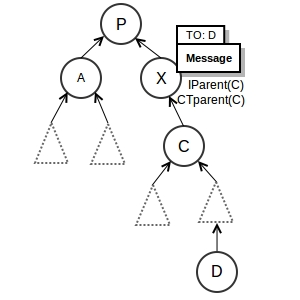
\includegraphics[width=.48\columnwidth]{Images/lb1.jpg}
            \label{fig:lb1}}
  \subfigure[]
  {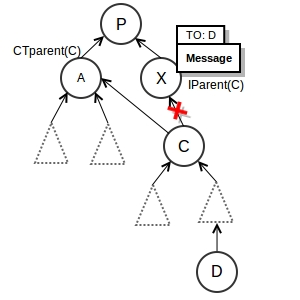
\includegraphics[width=.48\columnwidth]{Images/lb2.jpg}
                        \label{fig:lb2}}
                            \subfigure[]
  {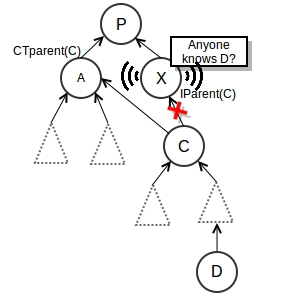
\includegraphics[width=.48\columnwidth]{Images/lb3.jpg}
            \label{fig:lb3}}
  \subfigure[]
  {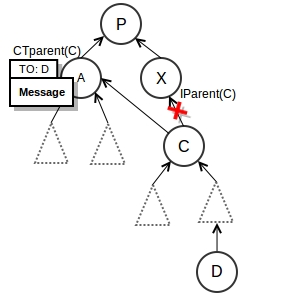
\includegraphics[width=.48\columnwidth]{Images/lb4.jpg}
    \label{fig:lb4}}
            \caption{Alternative top-down routing upon Ctree change.}\label{fig:localbroadcast}
\end{center}
\end{figure}


Consider the following scenario: node X receives a packet with destination IPv6
address D (see Figure \ref{fig:lb1}). After consulting its standard routing
table $IP-children_X$, X forwards the packet to C. However, the link X
$\Rightarrow$ C fails, for some reason, and C does not reply with an
acknowledgment.
Then, X makes a constant number (e.g., 30 times in CTP) of retransmission
attempts. Meanwhile, since node C also lost its connection to X, it decides to
change its parent in the collection tree to node A (see Figure \ref{fig:lb2}).
Having changed its parent, C starts sending beacons to A, which creates an entry
in its alternative routing table $RC-children_A$ for the subtree rooted at C, and
keeps it as long as it receives periodic beacons from C (which will be done as long as $CTparent_C$ = A).

Having received no acknowledgement from C, X activates the \textit{local
broadcast} mode: it sets the message's type to ``LB'' and broadcasts
it to all its one-hop neighbors (see Figure \ref{fig:lb3}). Upon
receiving the local broadcast, node A consults its alternative
routing table and finds out that the destination address D falls
within the IPv6 address range C. It then forwards the packet to C,
from where the packets follows along its standard route in the
subtree of C (see Figure \ref{fig:lb4}).

Note that this
mechanism does not guarantee that the message will be delivered. If no one-hop
neighbor of X had the address range of C in its alternative routing table, then
the packet would be lost. Nevertheless, we argue that the probability that the
message will be forwarded to the appropriate subtree is high.

\subsection{Alternative routing: geometric rationale}

The success of the local broadcast mechanism lies in the ability to forward
messages top down along the IPtree, in spite of one or more link or node
failures on the way.
Note that, whenever a node of IPtree is unavailable, it
might not be possible to find the right subtree of the destination.
Matrix is designed to handle (non-adjacent) link or node failures and relies on
a single local broadcast and temporary reverse collection links (RCtree).

Consider once again the scenario illustrated in Figure \ref{fig:localbroadcast}.
When a node X is unable to forward a packet to the next hop, it activates the
local broadcast mechanism, and it becomes essential that one of X's one-hop
neighbors (in this case A) has replaced X as a parent of C in
the collection tree. Therefore, given that the new parent of C is A, it becomes
essential that X and A are neighbors. We argue that it is unlikely that this is not the case.

\begin{figure}[!ht]
    \centering
    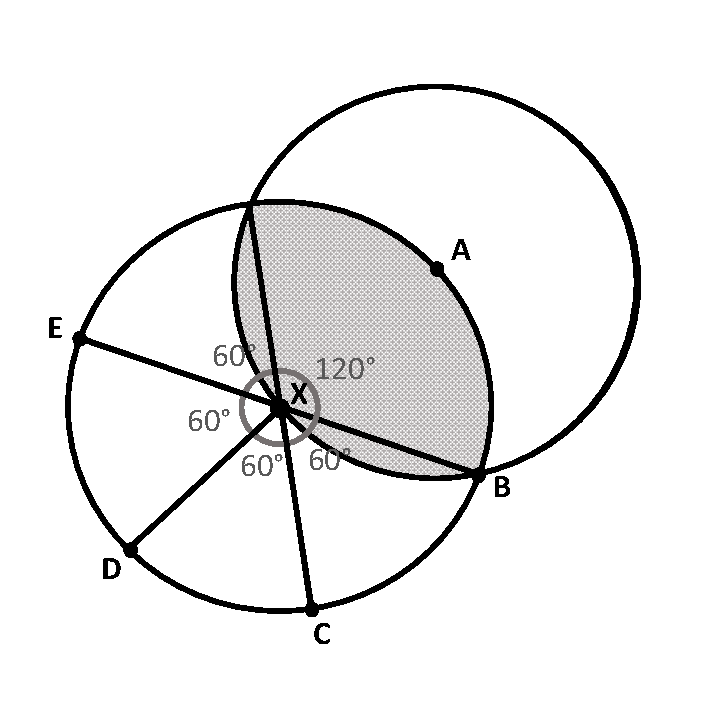
\includegraphics[width=.6\linewidth]{./Images/localbroad.pdf}
\caption{UDG model: the number of independent neighbors of X is at most 5.}
    \label{fig:udgIndN}
\end{figure}

Our argument is of geometric nature. Since the considered 6LoWPAN is
wireless, we show our argument in a unit disk graph (UDG) model
\cite{Clark:1991}. We use the fact that the number of independent neighbors of
any node in a UDG is bounded by a small constant, namely 5. The proof of this
fact is sketched in Figure \ref{fig:udgIndN}: consider a node X and its neighbor
A. Any node located inside the gray region is a neighbor of both X and A, so any
neighbor of X that is independent of (not adjacent to) A has to be outside the
gray area and inside the circle around X. Let's call this neighbor B. The next
independent neighbor of X has to be located outside the 60 degree sector that
starts at B, and so on. This procedure can be repeated no more than 5 times,
before the 360 degrees around X are covered.

Given that the maximum number of neighbors that do not know each
other is very small, for any possible node distribution and density
around X, the probability that two neighbors of X are independent is
low. In Figure \ref{fig:lb3}, since both X and A are neighbors of C,
the probability that they are themselves neighbors is high. Similar
arguments can be used to back the effectiveness of the local
broadcast mechanism when dealing with different non-adjacent link
and node failures.

Note that this reasoning is only valid in an open space without obstacles and,
even then, does not guarantee that the message will be delivered. Nevertheless,
our experiments show that this intuition is in fact correct, and Matrix has a
95\%--99\% message delivery success in scenarios with node failures of
increasing frequency and duration.